\section{Methods}\label{sec:method}

To solve the connector insertion tasks, we consider and evaluate a variety of RL algorithms.
% \subsection{Preliminaries}\label{sec:background}
% In a Markov decision process (MDP), an agent at every time step is at state $s_t \in \mathcal{S}$, takes actions $u_t \in \mathcal{U}$, receives a reward $r_t \in \mathbb{R}$, and the state evolves according to environment transition dynamics $p(s_{t+1}|s_t, u_t)$. The goal of reinforcement learning is to choose actions $u_t \sim \pi(u_t|s_t)$ to maximize the expected returns $\E[\sum_{t=0}^H \gamma^t r_t]$ where $H$ is the horizon and $\gamma$ is a discount factor. The policy $\pi(u_t|s_t)$ is often chosen to be an expressive parametric function approximator, such as a neural network, as we use in this work.

\subsection{Efficient Off-Policy Reinforcement Learning}
% One class of RL methods additionally estimates the expected discounted return after taking action $u$ from state $s$, the {Q-value} $Q(s, u)$. Q-values can be recursively defined with the Bellman equation:
% \begin{align}
%     Q(s_t, u_t) = \E_{s_{t+1}}[r_t + \gamma \max_{u_{t+1}} Q(s_{t+1}, u_{t+1})]
% \end{align}
% and learned from off-policy transitions $(s_t, u_t, r_t, s_{t+1})$. Because we are interested in sample-efficient real-world learning, we use such RL algorithms that can take advantage of off-policy data.

% For control with continuous actions, computing the required maximum in the Bellman equation is difficult. Continuous control algorithms such as deep deterministic policy gradients (DDPG) \citep{lillicrap2015continuous} additionally learn a policy $\pi_\theta(u_t|s_t)$ to approximately choose the maximizing action. 
In this paper we specifically consider two off-policy continuous control reinforcement learning algorithms that lend themselves well to real-world learning as they are sample efficient, stable, and require little hyperparameter tuning.

\textbf{Twin Delayed Deep Deterministic Policy Gradients (TD3).} 
Like DDPG, TD3 optimizes a deterministic policy \citep{fujimoto2018td3} but uses two Q-function approximators to reduce value overestimation \cite{vanhasselt2016doubledqn} and delayed policy updates to stabilize training.

\textbf{Soft Actor Critic (SAC).}
SAC is an off-policy value-based reinforcement learning method based on the maximum entropy reinforcement learning framework with a stochastic policy \citep{haarnoja2018sac}.

We used the implementation of these RL algorithms publicly available at \href{https://github.com/vitchyr/rlkit}{\texttt{rlkit}} \citep{pong2018tdm}.

\subsection{Residual Reinforcement Learning}

As discussed in chapter~\ref{chapter:residualrl}, instead of randomly exploring from scratch, we can inject prior information into an RL algorithm in order to speed up the training process, as well as to minimize unsafe exploration behavior. In residual RL, actions $u_t$ are chosen by additively combining a fixed policy $\pi_\text{H}(s_t)$ with a parametric policy $\pi_\theta(u_t|s_t)$:
\begin{equation}\label{eq:ctrl_seq}
    u_t = \pi_\text{H}(s_t) + \pi_\theta(s_t).
\end{equation}

The parameters $\theta$ can be learned using any RL algorithm. In this work, we evaluate both SAC and TD3, explained in the previous section.
% The residual RL implementation that we use in our experiments is summarized in Algorithm~\ref{alg:residualrl}.

% \begin{figure}
%     % \setlength{\textfloatsep}{0.09cm}
%     \begin{algorithm}[H]
%        	\caption{Residual reinforcement learning}
%        	\label{alg:residualrl}
%        	\begin{algorithmic}[1]
%         \REQUIRE policy $\pi_\theta$, hand-engineered controller $\pi_\text{H}$.
%         \FOR{$n=0,...,N-1$ episodes}
%             \STATE Sample initial state $s_0 \sim E$.
%             \FOR{$t=0,...,H -1$ steps}
%                 \STATE Get policy action $u_t \sim \pi_\theta(u_t|s_t)$.
%                 \STATE Get action to execute $u'_t = u_t + \pi_\text{H}(s_t)$.
%                 \STATE Get next state $s_{t+1} \sim p(\cdot \mid s_t, u'_t)$.
%                 \STATE Store $(s_t, u_t, s_{t+1})$ into replay buffer $\mathcal R$.
%                 \STATE Sample set of transitions $(s, u, s') \sim \mathcal R$.
%                 \STATE Optimize $\theta$ using RL with transitions.
%             \ENDFOR
%         \ENDFOR
%        	\end{algorithmic}
%     \end{algorithm}
%     % \setlength{\floatsep}{0.09cm}
%     \vspace{1cm}
% \end{figure}


A simple P-controller serves as the hand-designed controller $\pi_\text{H}$ of our experiments.  The P-controller operates in Cartesian space and calculates the current control action by 
\begin{equation}
\pi_\text{H}(s_t) = - k_p\cdot (x_t - x^{*}), 
\end{equation}
where $x^{*}$ denotes the commanded goal location. As control gains we use $k_p = [\,1, \,1,\, 0.3\,]$. This P-controller quickly centers the end-effector above the goal position and reaches the goal after about 10 time steps from the reset position, which is located 5cm above the goal.

\begin{figure}[ht!]
    \centering
    \resizebox{1.02\linewidth}{!}{
    \begin{subfigure}[b]{0.32\linewidth}
        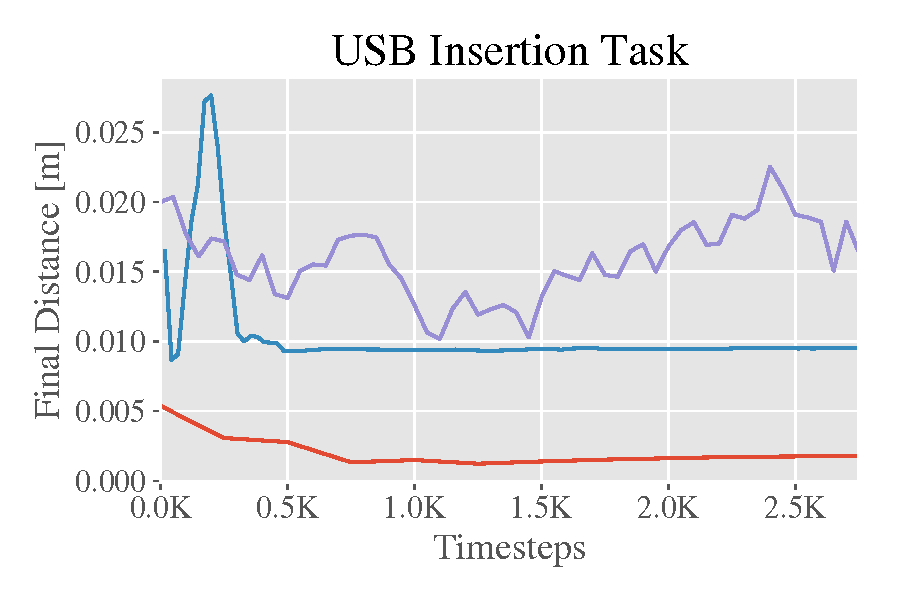
\includegraphics[width=0.99\linewidth]{insertion/newfigs/USB_images_distance.pdf}
    \end{subfigure}
    \begin{subfigure}[b]{0.32\linewidth}
        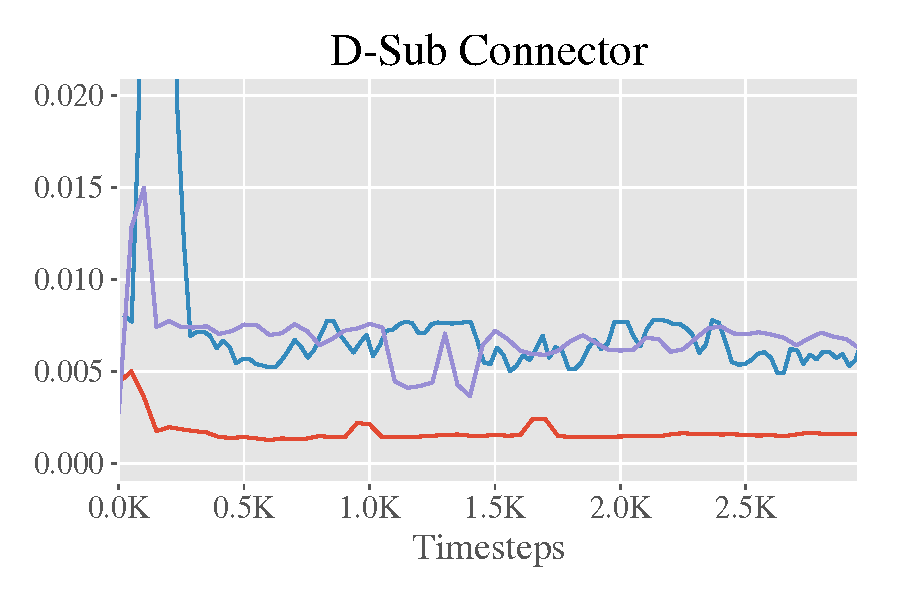
\includegraphics[width=0.99\linewidth]{insertion/newfigs/DSUB_images_distance.pdf}
    \end{subfigure}
    \begin{subfigure}[b]{0.32\linewidth}
        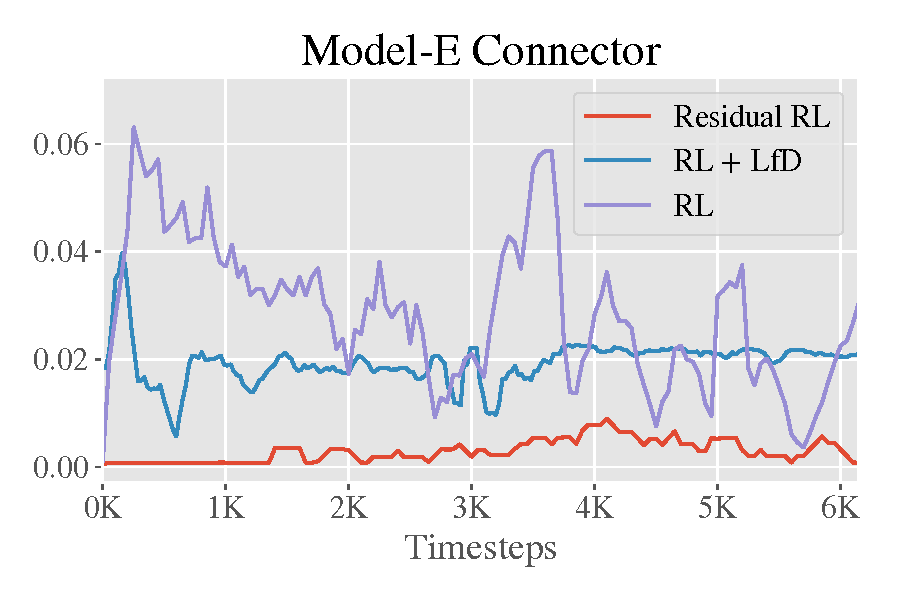
\includegraphics[width=0.99\linewidth]{insertion/newfigs/Waterproof_images_distance.pdf}
    \end{subfigure}
    }
    \caption{Resulting final mean distance during the vision-based training. The comparison includes RL, residual RL, and RL with learning from demonstrations. Only residual RL manages to deal with the high-dimensional input and consistently solve all the tasks after the given amount of training. The other methods learn to move downwards, but often get stuck in the beginning of the insertion and fail to recover from unsuccessful attempts.}
    \label{vision_based_distance_all}
    %\vspace{-0.5cm}
\end{figure}

%\pagebreak

\subsection{Learning from Demonstrations}

Another method to incorporate prior information is to use demonstrations from an expert policy to guide exploration during RL. We first collected demonstrations with a joystick controller. Then, we add a behavior cloning loss while performing RL that pushes the policy towards the demonstrator actions, as previously considered in \citep{nair2018demonstrations}. Instead of DDPG, the underlying algorithm RL algorithm used is TD3.


